\documentclass{article}
\usepackage{iclr2027_conference,times}
\usepackage[T1]{fontenc}
\usepackage{lmodern}
\usepackage{hyperref}
\usepackage{url}
\usepackage{booktabs}
\usepackage{microtype}
\usepackage{amsmath,amssymb,amsthm,mathtools}
\usepackage{xcolor}
\usepackage{enumitem}
\usepackage{tikz}
\usetikzlibrary{arrows.meta,decorations.pathreplacing,positioning}

\newtheorem{theorem}{Theorem}
\newtheorem{lemma}[theorem]{Lemma}
\newtheorem{proposition}[theorem]{Proposition}
\newtheorem{corollary}[theorem]{Corollary}
\newtheorem{remark}[theorem]{Remark}
\newcommand{\E}{\mathbb E}
\newcommand{\Pp}{\mathbb P}
\newcommand{\1}{\mathbf 1}
\newcommand{\N}{\mathbb N}
\newcommand{\Rad}{\operatorname{Rad}}
\newcommand{\KL}{\operatorname{KL}}
\newcommand{\TV}{\operatorname{TV}}
\newcommand{\poly}{\operatorname{poly}}

\title{The Statistical Price of Directed Neighborhoods}

\author{\textbf{Pahan Dewasurendra} \\ Johns Hopkins University}

\hypersetup{pdftitle={The Statistical Price of Directed Neighborhoods},pdfauthor={Pahan Dewasurendra},pdfkeywords={conditional averages, directed graphs, neighborhood learning, minimax rates, sample complexity, Caro-Wei inequality},pdfsubject={preprint}}
\begin{document}
\maketitle

\begin{abstract}
Conditional-average learning asks for the average target label in every graph neighborhood from
i.i.d. labeled vertices. Its recent combinatorial characterization leaves a logarithmic sample-
complexity gap: the upper bound contains
$\alpha_2\log(1/\epsilon)/\epsilon$, while the lower bound is only
$\alpha_2/(\epsilon\log\alpha_2)$. We determine exactly when the accuracy logarithm is real.

For undirected neighborhoods, we prove that the original empirical-neighborhood learner has
expected squared error at most
\[
 \frac{\alpha_1}{m+1}+\frac{7\alpha_2}{2m}.
\]
The proof integrates its pointwise variance through a measure-valued weighted Caro--Wei
inequality. This removes the logarithm without changing the algorithm, including on uncountable
domains. Conversely, for directed neighborhoods we construct $q$ disjoint transitive tournaments
and a single known alternating concept for which every learner suffers
$\Omega((q/m)\log(1+m/q))$ error with constant probability. The unknown object is only the
marginal distribution. Independent mass imbalances hidden in unsampled pairs accumulate over
nested suffixes, one harmonic scale at a time. A matching undirected lower bound follows from
disjoint edges.

Consequently, at constant confidence the worst-case sample complexity for parameters
$(\alpha_1,\alpha_2)=(d,q)$ is
$\Theta((d+q)/\epsilon)$ for undirected graphs and
$\Theta((d+q\log(1/\epsilon))/\epsilon)$ for directed graphs. A distribution-dependent
neighborhood-leverage quantity explains both rates. Thus edge direction causes a genuine
logarithmic statistical penalty even when the target concept is known, $\alpha_1=0$, and
$\alpha_2=1$.
\end{abstract}

\section{Introduction}

Many learning tasks ask not for the label of one point, but for an average over points judged
relevant to it. Examples include checking whether a local explanation is reliable, auditing subgroup
behavior, and estimating preferences over a recommendation neighborhood
\citep{ribeiro2018,bhattacharjee2024,hardt2016}. \citet{bressan2026} recently isolated this task as
\emph{conditional-average learning}. A known directed graph $G$ specifies a closed
out-neighborhood $N[x]$ for every instance $x$. From i.i.d. samples labeled by an unknown binary
concept $c$, a learner predicts
\begin{equation}
 s_c(x)=\E_{X'\sim D}[c(X')\mid X'\in N[x]]
 \label{eq:target}
\end{equation}
under integrated square loss.

Two joint graph--class parameters characterize learnability. The parameter $\alpha_1$ is the
largest independent set shattered by the concept class. For a fixed concept $c$, let $B_c$ contain
the vertices whose neighborhoods have both labels, and let $\alpha_2(G,c)$ be the independence
number of the graph induced by $B_c$. The class parameter $\alpha_2$ is the supremum over $c$.
Finiteness of $\alpha_1+\alpha_2$ is necessary and sufficient \citep{bressan2026}. Their quantitative
bounds, suppressing confidence for the moment, are
\begin{equation}
 \Omega\!\left(\frac{\alpha_1+\alpha_2/\log\alpha_2}{\epsilon}\right)
 \quad\text{and}\quad
 O\!\left(\frac{\alpha_1+\alpha_2\log(1/\epsilon)}{\epsilon}\right).
 \label{eq:old-gap}
\end{equation}
The upper logarithm arises by splitting neighborhood masses into dyadic levels. At every level,
light neighborhoods have small total mass but their empirical means have large variance. It was
unknown whether accumulating all levels is inherent.

We show that the answer is controlled by direction. In an undirected graph, symmetry couples
the mass of every vertex to the masses of vertices that count it as a neighbor. A weighted
independence inequality sums the inverse-neighborhood variances in one shot and eliminates all
dyadic levels. Direction breaks this charging argument. A one-way chain has independence number
one but has nested suffix neighborhoods at arbitrarily many mass scales. Independent uncertainties
at those scales accumulate harmonically.

\paragraph{Contributions.}
Our results are summarized in Table~\ref{tab:rates}.
\begin{table}[t]
\centering
\caption{Worst-case sample complexity at a universal constant confidence. Constants are universal.
The directed logarithm is read as $1+\log(1/\epsilon)$.}
\label{tab:rates}
\begin{tabular}{lcc}
\toprule
Neighborhoods & Previous bounds & This work \\
\midrule
Undirected & between \eqref{eq:old-gap} & $\Theta((\alpha_1+\alpha_2)/\epsilon)$ \\
Directed & between \eqref{eq:old-gap} & $\Theta((\alpha_1+\alpha_2\log(1/\epsilon))/\epsilon)$ \\
\bottomrule
\end{tabular}
\end{table}

First, we prove a sharp expected-risk upper bound for the existing learner on every measurable
undirected graph:
\[
 \E L(h_S)\le \frac{\alpha_1}{m+1}+\frac{7\alpha_2}{2m}.
\]
The central step is a weighted Caro--Wei inequality for probability measures. The finite weighted
inequality is classical and has stronger power-weighted forms in feedback-graph learning
\citep{caro1979,wei1981,eldowa2023}. The novelty is that its direct integration of the
conditional-average estimator removes the entire accuracy logarithm. An i.i.d. discretization
argument extends the inequality to arbitrary measurable domains.

Second, we prove that the directed logarithm is unavoidable in its strongest qualitative regime.
Our hard concept class is a singleton, so $\alpha_1=0$ and the learner knows every label before
sampling. On $q$ disjoint one-way chains, $\alpha_2=q$. The unknown marginal puts a fixed total
mass on each adjacent zero--one pair but hides an independent sign in its within-pair mass split.
Not observing a pair reveals exactly no information about its sign. Every suffix average contains
the sum of its missing signs. Averaging the resulting posterior variances over all suffixes produces
the harmonic number $H_s$ and risk $\Omega(q\log(1+m/q)/m)$. A Hilbert-space fourth-moment
argument upgrades Bayes expectation to a constant-probability minimax lower bound.

Third, a separate Assouad construction on $q$ undirected edges proves $\Omega(q/m)$ risk with a
known concept. Combining these constructions with ordinary PAC hardness gives the exact worst-case
envelopes in Table~\ref{tab:rates}. We also introduce a distribution-dependent neighborhood
leverage. It is at most $\alpha_2$ for undirected graphs and equals $\Theta(qH_s)$ on the hard
directed family, exposing the quantity that direction allows to grow.

\begin{figure}[t]
\centering
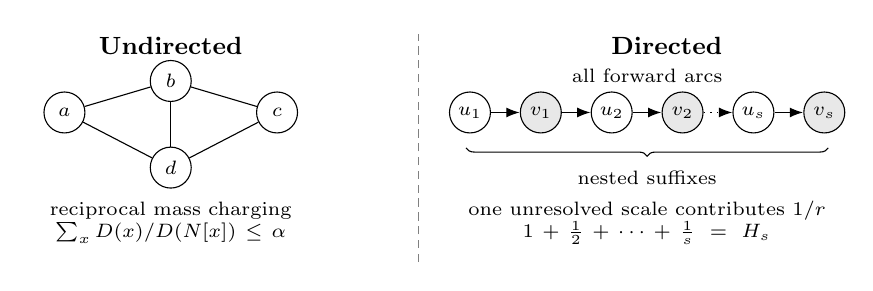
\begin{tikzpicture}[
  vertex/.style={circle,draw,inner sep=0pt,minimum size=5.2mm,font=\scriptsize},
  every edge/.style={line width=.45pt},
  >=Latex]
  \node[font=\small\bfseries] at (-3.15,1.2) {Undirected};
  \node[vertex] (a) at (-4.5,0.35) {$a$};
  \node[vertex] (b) at (-3.15,0.75) {$b$};
  \node[vertex] (c) at (-1.8,0.35) {$c$};
  \node[vertex] (d) at (-3.15,-0.35) {$d$};
  \draw (a)--(b)--(c);
  \draw (a)--(d)--(c);
  \draw (b)--(d);
  \node[align=center,font=\scriptsize,text width=3.4cm] at (-3.15,-1.05)
    {reciprocal mass charging\\$\sum_x D(x)/D(N[x])\le\alpha$};

  \draw[densely dashed,gray] (0,-1.55)--(0,1.35);
  \node[font=\small\bfseries] at (3.15,1.2) {Directed};
  \foreach \x/\lab/\col in {0.65/$u_1$/white,1.55/$v_1$/gray!18,2.45/$u_2$/white,
      3.35/$v_2$/gray!18,4.25/$u_s$/white,5.15/$v_s$/gray!18}{
    \node[vertex,fill=\col] at (\x,0.35) {\lab};
  }
  \draw[->] (0.92,0.35)--(1.28,0.35);
  \draw[->] (1.82,0.35)--(2.18,0.35);
  \draw[->] (2.72,0.35)--(3.08,0.35);
  \draw[->,dotted] (3.62,0.35)--(3.98,0.35);
  \draw[->] (4.52,0.35)--(4.88,0.35);
  \draw[decorate,decoration={brace,mirror,amplitude=3pt}]
      (0.6,-0.1)--(5.2,-0.1) node[midway,below=5pt,font=\scriptsize] {nested suffixes};
  \node[align=center,font=\scriptsize,text width=4.6cm] at (2.9,-1.05)
    {one unresolved scale contributes $1/r$\\$1+\frac12+\cdots+\frac1s=H_s$};
  \node[font=\scriptsize] at (2.9,0.82) {all forward arcs};
\end{tikzpicture}
\caption{Why direction changes the rate. Symmetry makes inverse-neighborhood charges share one
independence budget. A transitive directed chain supports nested suffixes at every mass scale, so
unseen pair imbalances accumulate harmonically.}
\label{fig:mechanism}
\end{figure}

\section{Setting and prior result}

Let $G=(\mathcal X,E)$ be a simple directed graph, with antiparallel edges allowed. Write
$N^+(x)=\{y:(x,y)\in E\}$ and $N[x]=N^+(x)\cup\{x\}$. A set $I$ is independent if no two
distinct vertices in $I$ have an edge in either direction. We assume the edge relation and all
functions used below are measurable. Let $\mathcal C\subseteq\{0,1\}^{\mathcal X}$ and
$D$ be a distribution on $\mathcal X$. A sample
$S=((X_1,c(X_1)),\ldots,(X_m,c(X_m)))$ is drawn i.i.d. from $D$ and an unknown
$c\in\mathcal C$. The learner returns $h_S:\mathcal X\to[0,1]$ and incurs
\[
 L_D(h_S)=\E_{X\sim D}(h_S(X)-s_c(X))^2,
\]
where $s_c$ is defined in \eqref{eq:target}. Closed neighborhoods have positive mass almost surely
under $X\sim D$, so the target is well defined where it is evaluated.

An independent set $I$ is shattered if
$|\{c|_I:c\in\mathcal C\}|=2^{|I|}$. Let $\alpha_1(G,\mathcal C)$ be the largest size of such
a set. A neighborhood is \emph{bichromatic} under $c$ if it contains both labels. Let $B_c$ be
the set of its centers and $G_c=G[B_c]$. Define
\[
 \alpha_2(G,c)=\alpha(G_c),\qquad
 \alpha_2(G,\mathcal C)=\sup_{c\in\mathcal C}\alpha_2(G,c).
\]
We abbreviate these parameters by $\alpha_1,\alpha_2$.

We use the learner of \citet{bressan2026}. If $S\cap N[x]$ is nonempty, it predicts the empirical
fraction of ones there. Otherwise it invokes the one-inclusion-graph predictor on the vertices that
are isolated in the graph induced by $S\cup\{x\}$. We need only two properties established in their
proof. For every $x$,
\begin{equation}
 \E_S(h_S(x)-s_c(x))^2\le \frac{7}{2mD(N[x])},
 \label{eq:pointwise}
\end{equation}
and the integrated contribution of isolated monochromatic neighborhoods is at most
$\alpha_1/(m+1)$. Nonisolated monochromatic neighborhoods incur zero loss. Their proof combines
\eqref{eq:pointwise} with a light-neighborhood lemma separately on $O(\log(1/\epsilon))$ mass
levels. We next avoid that partition when $G$ is undirected.

\section{Symmetry removes the accuracy logarithm}

We first state the measure-valued inequality that allows all neighborhood masses to be charged at
once. For an undirected graph $H=(V,F)$ and finite measure $\mu$, write
$\mu(N_H[x])=\int\1\{y\in N_H[x]\}\,d\mu(y)$.

\begin{lemma}[Measure-weighted Caro--Wei]\label{lem:measure-cw}
Let $H$ be a measurable undirected graph with finite independence number $\alpha(H)$ and let
$\mu$ be a finite measure on its vertices. Then
\begin{equation}
 \int \frac{1}{\mu(N_H[x])}\,d\mu(x)\le \alpha(H),
 \label{eq:measure-cw}
\end{equation}
with the integrand set to zero on the null set where the denominator vanishes.
\end{lemma}

For a finite atomic measure, \eqref{eq:measure-cw} is the weighted Caro--Wei inequality. Assigning
independent exponential clocks with rates equal to the atom masses proves it: vertices whose clocks
are smallest in their closed neighborhoods form an independent set, and the inclusion probability
of $x$ is its mass divided by its neighborhood mass. The non-atomic extension is not automatic,
since one cannot assign an independent clock measurably to every point. Our full proof instead
samples a finite graph from the measure and passes to a monotone limit. This also handles atoms and
repeated sampled points, as shown in Appendix~\ref{app:upper}.

\begin{theorem}[Undirected expected risk]\label{thm:undirected-upper}
Let $G$ be undirected and let $h_S$ be the conditional-average learner above. For every
$D$, $c\in\mathcal C$, and $m\ge1$,
\begin{equation}
 \E_S L_D(h_S)\le
 \frac{\alpha_1(G,\mathcal C)}{m+1}
 +\frac{7\alpha_2(G,c)}{2m}.
 \label{eq:undirected-risk}
\end{equation}
\end{theorem}

\begin{proof}
Only bichromatic and isolated monochromatic neighborhoods can contribute. For $x\in B_c$,
the closed neighborhood of $x$ in $G_c$ is contained in its closed neighborhood in $G$. Hence
\[
 D(N_G[x])\ge D(N_{G_c}[x]).
\]
Integrating \eqref{eq:pointwise} over $B_c$ and applying Lemma~\ref{lem:measure-cw} to the
restriction of $D$ to $B_c$ gives
\[
 \int_{B_c}\E_S(h_S(x)-s_c(x))^2dD(x)
 \le \frac{7}{2m}\int_{B_c}\frac{dD(x)}{D(N_{G_c}[x])}
 \le\frac{7\alpha(G_c)}{2m}.
\]
The prior one-inclusion leave-one-out argument bounds the isolated monochromatic contribution by
$\alpha_1/(m+1)$, and the remaining contribution is zero.
\end{proof}

The standard pointwise-median amplification in \citet{bressan2026} turns any expected squared-loss
bound $r$ into error $O(r)$ with failure probability $\delta$ using $O(\log(1/\delta))$ independent
runs. We therefore obtain the following immediate consequence.

\begin{corollary}[Undirected sample complexity]\label{cor:undirected-upper}
For undirected $G$, conditional averages are learnable with
\[
 m(\epsilon,\delta)=O\!\left(
 \frac{\alpha_1+\alpha_2}{\epsilon}\log\frac1\delta
 \right).
\]
At any fixed constant confidence, the rate is $O((\alpha_1+\alpha_2)/\epsilon)$.
\end{corollary}

The improvement is not a new algorithm. It is a structural fact about symmetric neighborhoods.
In the original dyadic proof, every light-mass level can spend the full independence budget. In an
undirected graph, Lemma~\ref{lem:measure-cw} forces all levels to share one budget.

\section{Direction forces harmonic accumulation}

We now show that no analogous conclusion holds for directed graphs. The construction is
distributional: the concept class contains one known function.

For integers $q,s\ge1$, take $q$ disjoint chains. Chain $a$ is ordered
\[
 u_{a,1},v_{a,1},u_{a,2},v_{a,2},\ldots,u_{a,s},v_{a,s},\ldots,
\]
and has an arc from every earlier vertex to every later vertex. There are no cross-chain arcs.
Let $c(u_{a,k})=0$ and $c(v_{a,k})=1$, and set $\mathcal C=\{c\}$. Then $\alpha_1=0$.
Every two vertices within a chain are adjacent in one direction. Every vertex except the last
supported one has a later opposite-labeled neighbor. Choosing one such vertex per chain shows
$\alpha_2=q$.

Fix $\eta=1/2$. For a sign array $\sigma\in\{-1,+1\}^{q\times s}$, define a marginal supported
on the first $s$ pairs by
\begin{equation}
 D_\sigma(u_{a,k})=\frac{1+\eta\sigma_{a,k}}{2qs},\qquad
 D_\sigma(v_{a,k})=\frac{1-\eta\sigma_{a,k}}{2qs}.
 \label{eq:paired-marginal}
\end{equation}
Every pair has sign-independent mass $1/(qs)$. At the first vertex of the suffix containing pairs
$k,\ldots,s$, of length $r=s-k+1$,
\begin{equation}
 s_c(u_{a,k})=\frac12-\frac{\eta}{2r}\sum_{\ell=k}^s\sigma_{a,\ell}.
 \label{eq:suffix-target}
\end{equation}
The cancellation in the denominator of \eqref{eq:suffix-target} is the purpose of pairing.

\begin{theorem}[Directed harmonic lower bound]\label{thm:directed-lower}
There are universal constants $c_0,c_1>0$ with the following property. For every $q\ge1$ and
$m\ge q$, the countable graph and singleton class above have $\alpha_1=0,\alpha_2=q$, and for
every possibly randomized learner there is a marginal $D_\sigma$ such that
\begin{equation}
 \Pp_S\!\left\{L_{D_\sigma}(h_S)
 \ge c_0\min\!\left(1,\frac{q}{m}\log\!\left(1+\frac mq\right)\right)\right\}
 \ge c_1.
 \label{eq:directed-lower}
\end{equation}
The concept and graph are known to the learner.
\end{theorem}

\paragraph{Proof idea.}
Set $s=\lceil m/q\rceil$ and give the signs in \eqref{eq:paired-marginal} independent Rademacher
priors. We make the experiment easier by revealing $\sigma_{a,k}$ whenever either member of pair
$(a,k)$ is sampled. Pair occupancy is independent of its sign, so every missing pair retains an
independent Rademacher sign.

Let $U_{a,r}$ be the number of missing pairs in the final $r$ pairs of chain $a$. From
\eqref{eq:suffix-target}, the posterior variance of the target at the first vertex of that suffix is
$\eta^2U_{a,r}/(4r^2)$. The mass of that vertex is at least $(1-\eta)/(2qs)$. Thus every predictor
has conditional posterior risk at least
\begin{equation}
 V=\frac{\eta^2(1-\eta)}{8qs}
 \sum_{a=1}^q\sum_{r=1}^s\frac{U_{a,r}}{r^2}.
 \label{eq:posterior-v}
\end{equation}
If a pair lies $t$ places from the chain end, its missing indicator has weight
$w_t=\sum_{r=t}^s r^{-2}$. Since $\sum_t w_t=H_s$, and each pair is missing with probability
$p=(1-1/(qs))^m\ge1/16$, we have $\E V\ge cH_s/s$. Missing indicators are negatively correlated
and $\sum_t w_t^2=O(1)$, so Paley--Zygmund gives $V\ge cH_s/s$ with constant probability.

It remains to turn posterior variance into actual error for an arbitrary, possibly biased predictor.
Restrict loss to the first vertex of every suffix and replace its sign-dependent mass by the lower
bound $(1-\eta)/(2qs)$. Conditioned on observed data, this lower bound is
$Q=\|A\xi-b\|^2$ in a fixed weighted Euclidean space, where $\xi$ contains the missing independent
signs. Hilbert-space Khintchine gives
\begin{equation}
 \E Q^2\le3(\E Q)^2.
 \label{eq:fourth}
\end{equation}
Since $\E Q\ge V$, another Paley--Zygmund application yields $Q\ge V/2$ with conditional
probability at least $1/12$. Averaging the sign prior then selects a deterministic $\sigma$.
Appendix~\ref{app:directed} gives all constants, handles nondivisibility, and proves
\eqref{eq:fourth}.

For $q=1$, the graph is a transitive tournament and both combinatorial dimensions are at most one.
Nonetheless its sample complexity is $\Omega(\log(1/\epsilon)/\epsilon)$. This corrects the
suppressed-log interpretation that tournaments are always $\widetilde O(1/\epsilon)$-easy: the
tilde hides a necessary factor.

\section{Matching envelopes and neighborhood leverage}

The undirected upper rate is also necessary. The proof uses $q$ disjoint edges and the same idea of
hiding mass rather than labels.

\begin{theorem}[Undirected lower bound]\label{thm:undirected-lower}
There are universal $c_2,c_3>0$ such that for every $q\ge1$ and $m\ge q$, there is an undirected
graph and singleton known concept with $\alpha_1=0,\alpha_2=q$ for which every learner has some
marginal $D$ satisfying
\[
 \Pp_S\{L_D(h_S)\ge c_2q/m\}\ge c_3.
\]
\end{theorem}

Take disjoint edges $\{u_i,v_i\}$, the known labels $c(u_i)=0,c(v_i)=1$, and
$D_\sigma(u_i)=(1+\eta\sigma_i)/(2q)$,
$D_\sigma(v_i)=(1-\eta\sigma_i)/(2q)$. The average on edge $i$ is
$(1-\eta\sigma_i)/2$. Neighboring sign experiments have $m$-sample KL divergence at most
$4m\eta^2/q$. Choosing $\eta$ proportional to $\sqrt{q/m}$ and applying Assouad's lemma leaves a
constant fraction of signs undecodable. Thresholding the learner's prediction at $1/2$ turns its
square loss into a decoder loss, yielding $\Omega(q/m)$. Appendix~\ref{app:undirected-lower}
gives a constant-probability version.

For prescribed $(d,q)$, append $d$ isolated vertices on which the class realizes all binary
labelings, while keeping it fixed on the hard component. This makes $\alpha_1=d$ and
$\alpha_2=q$. A marginal supported on the isolated vertices gives the classical
$\Omega(d/\epsilon)$ PAC lower bound \citep{ehrenfeucht1989}. Supporting it on the hard component
gives Theorem~\ref{thm:directed-lower} or \ref{thm:undirected-lower}. The larger lower bound is at
least half their sum.

\begin{corollary}[Price of direction]\label{cor:envelope}
Fix a universal confidence $1-\delta_0$. Among problems with
$(\alpha_1,\alpha_2)=(d,q)$, the worst-case sample complexity is
\[
 \Theta\!\left(\frac{d+q}{\epsilon}\right)
 \quad\text{for undirected graphs},\qquad
 \Theta\!\left(\frac{d+q\log(1/\epsilon)}{\epsilon}\right)
 \quad\text{for directed graphs}.
\]
\end{corollary}

A distribution-dependent quantity explains the split. On a countable domain define
\begin{equation}
 \Lambda_D(G,c)=\sum_{x\in B_c}\frac{D(x)}{D(N[x])}.
 \label{eq:leverage}
\end{equation}
Equation~\eqref{eq:pointwise} immediately gives
\begin{equation}
 \E L_D(h_S)\le\frac{\alpha_1}{m+1}+\frac{7\Lambda_D(G,c)}{2m}.
 \label{eq:leverage-risk}
\end{equation}
For undirected graphs, Lemma~\ref{lem:measure-cw} says $\Lambda_D\le\alpha_2$. On each hard
directed chain, the mass of a suffix of $r$ pairs is $r/(qs)$, while each first vertex has mass
$\Theta(1/(qs))$. Hence $\Lambda_D=\Theta(qH_s)$. The lower bound matches
\eqref{eq:leverage-risk} at the sample-dependent hard scale $s\asymp m/q$.

\section{Related work}

\paragraph{Conditional averages and local auditing.}
\citet{bressan2026} introduced conditional-average learning, proved its exact learnability
characterization, and obtained \eqref{eq:old-gap}. Their lower bound already shows that marginal
uncertainty can make a known concept hard, using bichromatic witnesses and degree binning. Our
paired construction avoids degree binning and instead makes nested directed neighborhoods collect
uncertainty at every scale. Their discussion notes that the light-neighborhood lemma is related to
weighted Caro--Wei in the undirected case, but it does not derive the integrated inequality or the
improved rate. Auditing local explanations also depends inversely on neighborhood locality
\citep{bhattacharjee2024}. That task estimates one global auditing functional of supplied
explanations, whereas conditional-average learning predicts every local mean.

\paragraph{Feedback graphs.}
Inverse-neighborhood sums are central in online learning with graph feedback. Directed graphs admit
bounds with logarithmic factors \citep{alon2015}. For undirected graphs,
\citet{eldowa2023} prove the stronger power-weighted inequality
$\sum_v p(v)^{1+b}/p(N[v])\le\alpha^{1-b}$. Its $b=0$ case contains finite weighted
Caro--Wei and our combinatorial step. Their application is online regret and they identify directed
feedback as substantially harder. Our contribution transfers the inequality to conditional-average
risk on general measure spaces and proves that direction changes the minimax accuracy rate.
Stochastic feedback graphs use different weighted independence and domination parameters based on
edge-observation probabilities \citep{esposito2022}.

\paragraph{Aggregate labels and conditional means.}
Learning from label proportions observes bag averages and predicts individual labels, reversing the
information flow considered here. Recent work gives near-optimal variance-reduced ERM and SGD
bounds in that setting \citep{busafekete2025}. Plug-in conditional-mean estimation and adaptive
nearest-neighbor classification require geometric or function-class control absent from arbitrary
neighborhood graphs \citep{grunewalder2018,balsubramani2019}.

\section{Discussion}

The separation isolates a structural cost, not an algorithmic artifact. Symmetry enforces reciprocal
mass accounting. Direction permits many centers to charge the same downstream mass at different
scales. The one-way chain is the extremal elementary example: its directed independence number is
one, but its neighborhood leverage is harmonic.

Our exact envelopes hold at constant confidence. Combining Theorem~\ref{thm:undirected-upper}
with median amplification gives the stated $\log(1/\delta)$ multiplier, while the existing general
lower bound supplies $\Omega(\log(1/\delta)/\epsilon)$ \citep{bressan2026}. We do not close the
optimal joint dependence on vanishing $\delta$. We also analyze squared loss. Other losses change
the pointwise mean-estimation rate and may produce a different price for nesting.

The lower graph is deliberately order-like, not pathological in size or computation. Its
neighborhoods encode queries such as ``average outcome among people at least this old,'' an example
already used to motivate directed conditional averages \citep{bressan2026}. The result says that
uniformly accurate local auditing of many nested threshold groups pays a logarithm even when the
outcome function is public. If neighborhoods represent symmetric similarity instead, the logarithm
vanishes.

\section*{Reproducibility statement}

All claims are nonasymptotic and all proofs are included after the references. The supplementary
artifact contains a short audit program. It exhaustively enumerates small paired-chain samples to
check the posterior-variance identity, verifies the harmonic weights, enumerates the
constant-probability occupancy step, checks the shifted Rademacher fourth-moment inequality, and
tests weighted Caro--Wei against exact independence numbers on random small graphs. The program
checks the derivations and is not used as an assumption.

\bibliography{references}
\bibliographystyle{iclr2027_conference}

\appendix
\section{Measure-valued weighted Caro--Wei}\label{app:upper}

We prove Lemma~\ref{lem:measure-cw} without requiring a jointly measurable family of independent
random clocks on an uncountable domain.

\begin{proof}[Proof of Lemma~\ref{lem:measure-cw}]
The claim is invariant to scaling $\mu$, so suppose first that $\mu$ is a probability measure.
Draw $Z_1,\ldots,Z_k$ independently from $\mu$. Construct a finite undirected graph on indices
$[k]$ by joining $i\ne j$ when $Z_i=Z_j$ or $Z_i$ and $Z_j$ are adjacent in $H$. Any independent
set of indices maps injectively to an independent set in $H$, so this sampled graph has independence
number at most $\alpha(H)$.

The ordinary Caro--Wei inequality applied conditionally on the sampled graph gives
\[
 \sum_{i=1}^k\frac{1}{1+d_i}\le\alpha(H),
\]
where $d_i$ is the degree of index $i$. Given $Z_i=x$, the closed-neighborhood count
$1+d_i$ has distribution $1+Y$ for
$Y\sim\operatorname{Bin}(k-1,p_x)$ and $p_x=\mu(N_H[x])$. Direct integration yields
\[
 \E\frac{1}{1+Y}
 =\int_0^1(1-p_x+p_xt)^{k-1}dt
 =\frac{1-(1-p_x)^k}{kp_x}.
\]
Taking expectation, summing the $k$ equal terms, and using measurability gives
\[
 \int f_k(p_x)\,d\mu(x)\le\alpha(H),\qquad
 f_k(p)=\begin{cases}[1-(1-p)^k]/p,&p>0,\\ k,&p=0.\end{cases}
\]
The functions $f_k$ increase pointwise to $1/p$ for $p>0$ and to infinity for $p=0$. Monotone
convergence therefore shows at once that the set $\{x:p_x=0\}$ is $\mu$-null and that the limiting
integral is at most $\alpha(H)$. For a finite nonzero measure, normalize by its total mass. The zero
measure is trivial.
\end{proof}

\begin{remark}
For a finite atomic measure, an equivalent proof assigns an independent exponential clock of rate
$\mu(x)$ to each positive-mass vertex. The set of vertices whose clock is smallest in its closed
neighborhood is independent and has expected size equal to the left side of
\eqref{eq:measure-cw}.
\end{remark}

\section{Directed lower bound}\label{app:directed}

We give a complete proof of Theorem~\ref{thm:directed-lower}. It suffices to consider deterministic
learners because independent learner randomness can be conditioned upon throughout.

\subsection{Posterior variance and harmonic weights}

Fix $q,m$ and set $s=\lceil m/q\rceil$, $n=qs$. Then $m\le n<m+q\le2m$ when $m\ge q$.
Use the marginal family \eqref{eq:paired-marginal} with $\eta=1/2$ and put the uniform prior on its
$n$ signs. Augment the observation by revealing the sign of a pair whenever either endpoint is
sampled. This can only decrease the minimax risk.

The total probability of every pair is $1/n$, independent of its sign. Thus the sequence of pair
indices in the sample is i.i.d. uniform on $[n]$, independent of all signs. Conditional on these
indices and the revealed signs, signs of unobserved pairs remain independent Rademachers.

For chain $a$, index suffixes by their number $r\in[s]$ of pairs. Let $U_{a,r}$ be the number of
unobserved pairs in that suffix. Equation~\eqref{eq:suffix-target} shows that its random part at
the first vertex is
\[
 -\frac{\eta}{2r}\sum_{j\in M_{a,r}}\sigma_j,
\]
where $M_{a,r}$ is the missing set. Its posterior variance is $\eta^2U_{a,r}/(4r^2)$. Also
$D_\sigma(u_{a,k})\ge(1-\eta)/(2n)$. Restricting the population loss to these first vertices proves
the conditional variance lower bound \eqref{eq:posterior-v}.

Let
\[
 w_t=\sum_{r=t}^s\frac1{r^2},\qquad
 Z=\sum_{a=1}^q\sum_{t=1}^s w_t I_{a,t},
\]
where $I_{a,t}$ indicates that the pair $t$ places from the end of chain $a$ is missing. Exchanging
the order of summation gives
\begin{equation}
 \sum_{a=1}^q\sum_{r=1}^s\frac{U_{a,r}}{r^2}=Z,
 \qquad
 \sum_{t=1}^s w_t=\sum_{r=1}^s\frac{r}{r^2}=H_s.
 \label{eq:weight-identities}
\end{equation}
Furthermore $w_t\le t^{-2}+\int_t^\infty x^{-2}dx\le2/t$, hence
$\sum_tw_t^2\le2\pi^2/3$.

Every pair is absent with probability $p=(1-1/n)^m$. For $n\ge m\ge1$, $p\ge1/4$ except when
$n=m=1$. For distinct pairs,
\[
 \E[I_iI_j]=(1-2/n)^m\le(1-1/n)^{2m}=p^2,
\]
so their covariance is nonpositive. Consequently
\[
 \E Z=q pH_s,
 \qquad
 \E Z^2\le(\E Z)^2+p q\sum_tw_t^2
 \le(\E Z)^2+\frac{2\pi^2pq}{3}.
\]
Since $q\ge1$, $p\ge1/4$, and $H_s\ge1$, Paley--Zygmund implies
\begin{equation}
 \Pp\{Z\ge \E Z/2\}
 \ge\frac{1}{4}\frac{(\E Z)^2}{\E Z^2}
 \ge c_{\rm occ}
 \label{eq:occupancy-pz}
\end{equation}
for a universal $c_{\rm occ}>0$. On this event,
\begin{equation}
 V\ge \frac{\eta^2(1-\eta)p}{16}\frac{H_s}{s}
 \ge c\frac{H_s}{s}.
 \label{eq:v-event}
\end{equation}

\subsection{A shifted Rademacher small-ball lemma}

\begin{lemma}\label{lem:shifted-smallball}
Let $\xi_1,\ldots,\xi_N$ be independent Rademachers, let $v_1,\ldots,v_N,b$ lie in a real
Hilbert space, and put $Y=\sum_i\xi_iv_i$ and $Q=\|Y-b\|^2$. Then
\[
 \E Q^2\le3(\E Q)^2,
 \qquad
 \Pp\{Q\ge\E Q/2\}\ge1/12.
\]
\end{lemma}

\begin{proof}
Write $v=\E\|Y\|^2=\sum_i\|v_i\|^2$ and $B=\|b\|^2$. The Hilbert-space fourth-moment
inequality gives $\E\|Y\|^4\le3v^2$. One direct proof expands the fourth power: terms with an
index of odd multiplicity vanish, while each surviving cross term is bounded by the corresponding
product of squared norms. Also
$\E\langle Y,b\rangle^2=\sum_i\langle v_i,b\rangle^2\le vB$.
Symmetry makes all cubic terms vanish. Expanding $Q^2$ therefore gives
\[
 \E Q^2
 =\E\|Y\|^4+B^2+4\E\langle Y,b\rangle^2+2Bv
 \le3v^2+B^2+6Bv
 \le3(v+B)^2.
\]
Since $\E Q=v+B$, the first claim follows. Paley--Zygmund applied to the nonnegative variable
$Q$ with threshold $1/2$ gives the second.
\end{proof}

Condition on sample pair indices, revealed signs, and learner randomness. The vector of all target
values at the first suffix vertices is an affine image of the missing independent signs. Define $Q$
by weighting the squared errors on those vertices uniformly by the lower bound
$(1-\eta)/(2n)$. The actual population error dominates $Q$, while
$Q=\|A\xi-b\|^2$ in a fixed weighted Euclidean space. Its conditional expectation is at least the
integrated posterior variance $V$. By
Lemma~\ref{lem:shifted-smallball}, $Q\ge V/2$ with conditional probability at least $1/12$.
Combining with \eqref{eq:occupancy-pz} and \eqref{eq:v-event} gives joint probability at least
$c_{\rm occ}/12$ that
\[
 L_{D_\sigma}(h_S)\ge c\frac{H_s}{s}.
\]
This probability is averaged over the uniform sign prior. Hence some deterministic $\sigma$ has
the same frequentist lower bound. Finally,
$H_s/s\ge c\min\{1,(q/m)\log(1+m/q)\}$ because $s=\lceil m/q\rceil$. This proves
Theorem~\ref{thm:directed-lower} except at $q=m=1$. At that endpoint, use the same two marginals
on the first pair without revealing its sign. Their one-sample total variation is $\eta<1$, while
their conditional averages differ by $\eta$. Le Cam's two-point argument gives a universal
constant-probability constant-risk lower bound, which is the required right side of
\eqref{eq:directed-lower} after changing constants.

\subsection{Inverting the risk lower bound}

For completeness, the condition
$m<cq\log(1/\epsilon)/\epsilon$ with a sufficiently small universal $c$ implies
$(q/m)\log(1+m/q)>c'\epsilon$ for all sufficiently small $\epsilon$. Bounded values of
$\epsilon$ are absorbed by changing constants. Thus Theorem~\ref{thm:directed-lower} implies
$\Omega(q\log(1/\epsilon)/\epsilon)$ constant-confidence sample complexity.

\section{Undirected lower bound}\label{app:undirected-lower}

We prove Theorem~\ref{thm:undirected-lower}. For the nontrivial regime $m\ge q$, fix
$\eta=a\sqrt{q/m}\le1/2$ for a sufficiently small universal $a$. Put the uniform prior on
$\sigma\in\{-1,+1\}^q$. Recall that the two endpoints of edge $i$ both have target
$\theta_i=(1-\eta\sigma_i)/2$.

For sign arrays differing only at coordinate $i$, the one-sample KL divergence is
\begin{align*}
 \KL(D_\sigma\|D_{\sigma^{(i)}})
 &=\frac{\eta}{q}\log\frac{1+\eta}{1-\eta}
 \le\frac{4\eta^2}{q}.
\end{align*}
Tensorization and Pinsker give
\[
 \TV(D_\sigma^m,D_{\sigma^{(i)}}^m)
 \le\sqrt{2m\eta^2/q}\le \sqrt2a.
\]
Choose $a\le1/(4\sqrt2)$. Assouad's argument then shows that for every decoder
$\widehat\sigma$,
\begin{equation}
 \E_{\sigma,S}d_H(\widehat\sigma,\sigma)\ge\frac{3q}{8}.
 \label{eq:assouad}
\end{equation}

Given a predictor $h$, decode $\widehat\sigma_i=+1$ if the average of $h(u_i)$ and $h(v_i)$ is
below $1/2$, and $-1$ otherwise. If this decoder errs, convexity gives
\[
 (h(u_i)-\theta_i)^2+(h(v_i)-\theta_i)^2\ge\frac{\eta^2}{2}.
\]
Every endpoint has mass at least $(1-\eta)/(2q)\ge1/(4q)$, so
\begin{equation}
 L_{D_\sigma}(h)\ge\frac{\eta^2}{8q}
 d_H(\widehat\sigma,\sigma).
 \label{eq:hamming-to-risk}
\end{equation}
Equations \eqref{eq:assouad}--\eqref{eq:hamming-to-risk} give Bayes expected risk at least
$3\eta^2/64=\Omega(q/m)$.

To obtain a probability statement, one may use a direct bounded-Hamming argument. Since
$0\le d_H\le q$ and its mean is at least $3q/8$,
\[
 \Pp\{d_H\ge3q/16\}\ge
 \frac{(3/8)-(3/16)}{1-(3/16)}=\frac3{13}.
\]
Together with \eqref{eq:hamming-to-risk}, the joint prior-and-sample probability of risk
$\Omega(q/m)$ is at least $3/13$. Averaging selects one deterministic $\sigma$. If $m<q$, set
$\eta$ to a small constant and apply the same proof to obtain constant risk, completing the stated
$\min\{1,q/m\}$ form.

\section{Auxiliary audits}

The supplementary program implements the following independent checks.
\begin{enumerate}[leftmargin=*,itemsep=2pt]
\item It enumerates every sample-location sequence for small $(q,s,m)$ and confirms
$\E V=pH_s/(4s)$ for the simpler uniform-label version of the chain calculation.
\item It verifies $\sum_tw_t=H_s$ and the uniform square-sum bound through $s=999$.
\item It enumerates all occupancy patterns induced by samples for small chains and checks the
constant-probability threshold in \eqref{eq:occupancy-pz}.
\item It enumerates Rademacher signs for random linear maps and shifts and checks
$\E Q^2\le3(\E Q)^2$.
\item It compares the weighted Caro--Wei sum with an exact exhaustive computation of the
independence number on random undirected graphs up to eight vertices and weights spanning six
orders of magnitude.
\item It exhausts the actual paired marginals and verifies their normalization, suffix targets,
posterior-variance identity, and the neighboring KL formula used in the edge lower bound.
\end{enumerate}


\end{document}
